\documentclass{article}

\usepackage[table, xcdraw]{xcolor}
\usepackage{graphicx} % Required for inserting images
\usepackage[most]{tcolorbox}
\usepackage[margin=1in]{geometry}
\usepackage{enumitem}
\usepackage{amsmath}
\usepackage{float}
\usepackage[normalem]{ulem}
\usepackage{cancel}
\usepackage{multirow}
\usepackage{titlesec}
\usepackage{tabto}
\usepackage{siunitx}
\usepackage{fancyhdr, lastpage}
\usepackage[utf8]{inputenc} % Required for inputting international characters
\usepackage[T1]{fontenc} % Output font encoding for international characters
\usepackage{mathpazo} % Palatino font

\pagestyle{fancy}
\lhead{Electronics I: Experiment \#1}
\rhead{Xaria Davis}
\cfoot{Page \thepage\ of \pageref{LastPage}}

\graphicspath{{Screenshots/}}

\renewcommand{\thesubsection}{\arabic{subsection}}
\titleformat{\subsubsection}[runin]
  {\normalfont\normalsize\bfseries}{\thesubsubsection}{1em}{}
  

\begin{document}

	% ======= Title Page ======== %
	\begin{titlepage} % Suppresses displaying the page number on the title page and the subsequent page counts as page 1
		\newcommand{\HRule}{\rule{\linewidth}{0.5mm}} % Defines a new command for horizontal lines, change thickness here
		
		\center % Center everything on the page
		
		%------------------------------------------------
		%	Headings
		%------------------------------------------------
		
		\textsc{\LARGE University of Central Florida}\\[1.5cm] % Main heading such as the name of your university/college
		
		\textsc{\Large Electronics I Lab}\\[0.5cm] % Major heading such as course name
		
		\textsc{\large Section 0014}\\[0.5cm] % Minor heading such as course title
		
		%------------------------------------------------
		%	Title
		%------------------------------------------------
		
		\HRule\\[0.4cm]
		
		{\huge\bfseries Experiment \# 1: Name of Experiment}\\[0.4cm] % Title of your document
		
		\HRule\\[1.5cm]
		
		%------------------------------------------------
		%	Author(s)
		%------------------------------------------------
		
		\begin{minipage}{0.4\textwidth}
			\begin{flushleft}
				\large
				\textit{Author}\\
				\textsc{Xaria Davis} % Your name
			\end{flushleft}
		\end{minipage}
		~
		\begin{minipage}{0.4\textwidth}
			\begin{flushright}
				\large
				\textit{Laboratory Partner}\\
				\textsc{Insert Name Here} % Lab Partner’s Name
			\end{flushright}
		\end{minipage}
		
		% If you don't want a lab partner, uncomment the two lines below and comment the code above
		%{\large\textit{Author}}\\
		%John \textsc{Smith} % Your name
		
		%------------------------------------------------
		%	Date
		%------------------------------------------------
		
		\vfill\vfill\vfill % Position the date 3/4 down the remaining page
		
		{\large\ February 22, 2023 } % Date, change the \today to a set date if you want to be precise
		
		%------------------------------------------------
		%	Logo
		%------------------------------------------------
		
		%\vfill\vfill
		%\includegraphics[width=0.2\textwidth]{placeholder.jpg}\\[1cm] % Include a department/university logo - this will require the graphicx package
		 
		%----------------------------------------------------------------------------------------
		
		\vfill % Push the date up 1/4 of the remaining page
		
	\end{titlepage}
	% =========================== %
	
	\section*{Preliminary Information}
		\subsubsection*{Date and time data was taken}
    		\tab Thursday, February 9, 2023 from 9am to 12pm
    
    \section*{Pre-labaratory Results}
 
 
    \pagebreak
    \section*{Experimental Procedure}


	\pagebreak
	\section*{Calculations and Simulations}
		\subsection*{Calculations for Fig. 1b and Fig. 3}
			Example images included below.
			
		\subsection*{Simulations for Fig. 3}
			% Fig. 3 schematic
			\begin{figure}[H]
		    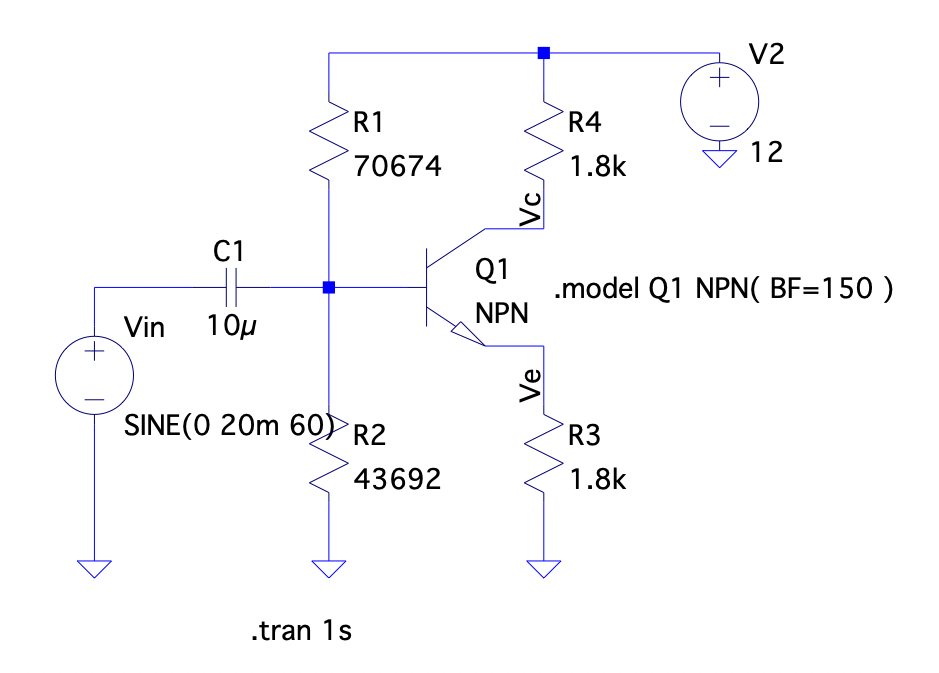
\includegraphics[width=12cm]{Fig 3 Schematic}
		    \centering
		    \caption{Schematic for Fig. 3}
		    \end{figure}
		    
			% Fig. 3 wave
			\begin{figure}[H]
		    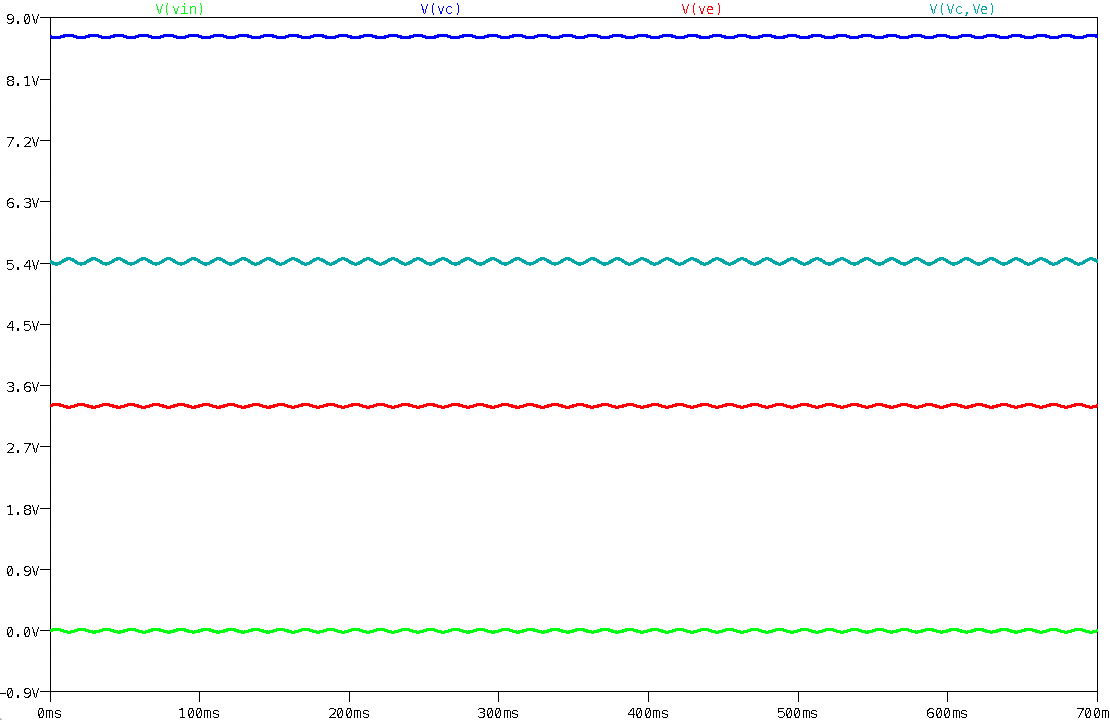
\includegraphics[width=12cm]{Fig 3 Wave}
		    \centering
		    \caption{Waveform for Fig. 3 voltages: $V_{in}, V_{E}, V_{C}, V_{CE}$}
		    \end{figure}

		    
	\pagebreak
	\section*{Plots and Waveforms}
		% Fig 3 Wave
		\begin{figure}[H]
	    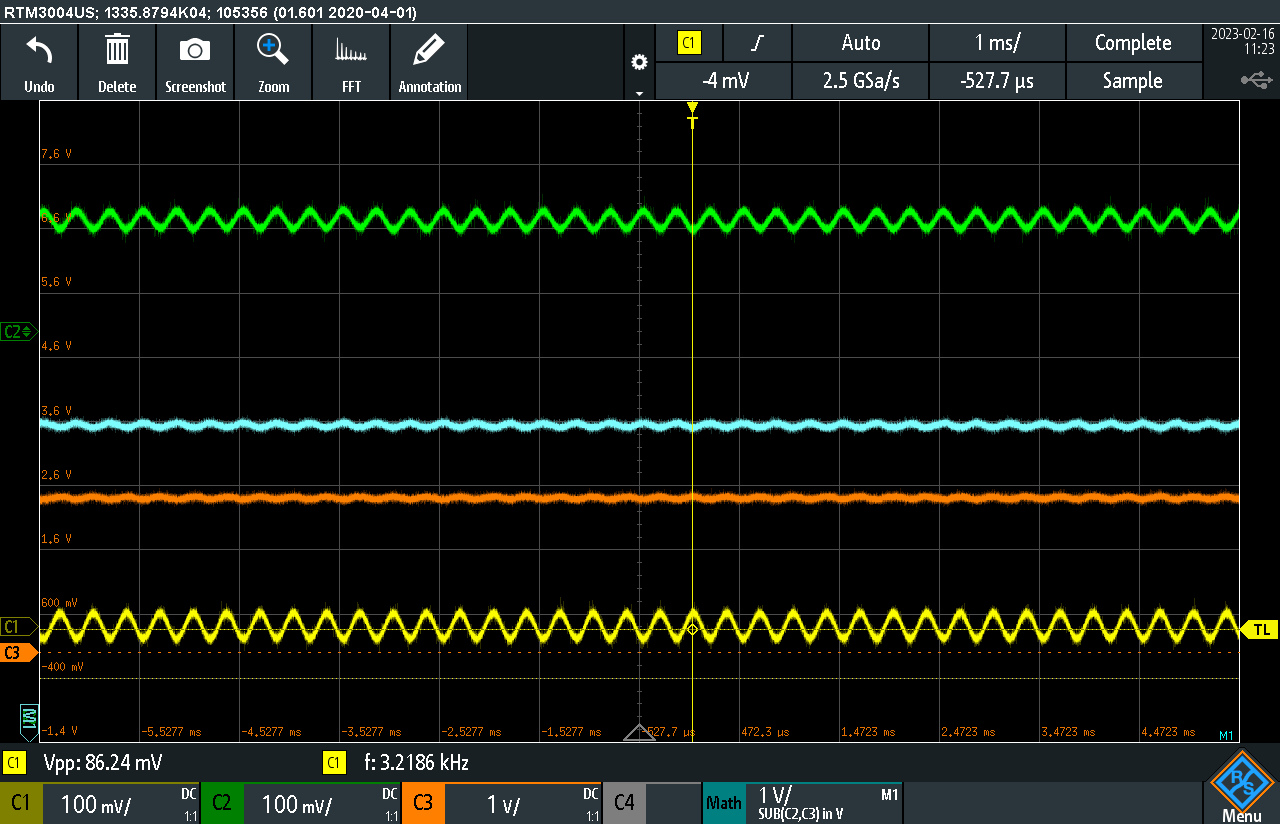
\includegraphics[width=14.9cm]{Oscilloscope}
	    \centering
	    \caption{Waveforms given by the oscilloscope for $V_{in}, V_{E}, V_{C}, V_{CE}$.}
	    \end{figure}
		
		
	\pagebreak	    
	\section*{Conclusion}
		
\end{document}